
\section{Hit-and-Run}

The ball walk does not mix rapidly from all starting points in arbitrary
convex bodies. While this hurdle can be overcome by starting with
a deep point and carefully maintaining a warm start, it is natural
to ask if there is a simple process that truly does mix rapidly from
any starting point. Hit-and-Run satisfies this requirement.

\begin{figure}[h]
\centering{}\includegraphics[width=0.7\textwidth]{Figures/Section_10\lyxdot 1}\caption{Hit-and-Run Algorithm}
\end{figure}

\begin{algorithm2e}[H]

\caption{$\mathtt{Hit\mbox{-}and\mbox{-}Run}$}

\SetAlgoLined

Input: starting point $x_{0}$ in a convex body $K$.

Repeat $T$ times: at current point $x$,
\begin{enumerate}
\item Pick a uniform random direction $\ell$ through $x$.
\item Go to a uniformly random point $y$ on the chord of $K$ induced by
$\ell$.
\end{enumerate}
\Return $x$.

\end{algorithm2e}

Since hit-and-run is a symmetric Markov chain, the uniform distribution
on $K$ is stationary for it. To sample from a general density proportional
to $f(x)$, in Step 2, we sample $y$ according to the density proportional
to $f$ restricted to the random line $\ell$. 
\begin{xca}
Show that Hit-and-Run satisfies detailed balance. 
\end{xca}

Next we give a formula for the next step distribution from a point
$u$.
\begin{lem}
\label{lem:har-next-step}The next step distribution of Hit-and-Run
from a point $u$ is given by
\[
P_{u}(A)=\frac{2}{\vol(S^{n-1})}\int_{A}\frac{dx}{\norm{x-u}^{n-1}\ell(u,x)}
\]
where $A$ is any measurable subset of $K$ and $\ell(u,x)$ is the
length of the chord in $K$ through $u$ and $x$.

\begin{figure}[h]
\begin{centering}
\includegraphics[width=0.7\textwidth]{Figures/Lemma_10\lyxdot 35}
\par\end{centering}
\end{figure}
\end{lem}

\begin{xca}
Prove Lemma \ref{lem:har-next-step}.
\end{xca}

The main theorem of this section is the following \cite{LV3}.

\begin{figure}[h]
\begin{centering}
\includegraphics[width=0.6\textwidth]{Figures/Thrm_10\lyxdot 37}\caption{Hit-and-Run from a corner}
\par\end{centering}
\end{figure}

\begin{thm}
\cite{LV3}\label{thm:har-cond} The conductance of Hit-and-Run in
a convex body $K$ containing the unit ball and of diameter $D$ is
$\Omega(1/(nD))$.
\end{thm}

This implies a mixing time of $O\left(n^{2}D^{2}\log(M/\varepsilon)\right)$
to get to within distance $\varepsilon$ of the target density starting
from an $M$-warm initial density. By taking one step from the initial
point, we can bound $M$ by $(D/d)^{n}$ where $d$ is the minimum
distance of the starting point from the boundary. Hence this gives
a bound of $\tilde{O}(n^{3}D^{2})$ from \emph{any} interior starting
point.

The proof of the theorem follows the same high-level outline as that
of the ball walk, needing two major ingredients, namely, one-step
coupling and isoperimetry. Notably, the isoperimetry is for a non-Euclidean
notion of distance. We begin with some suitable definitions. 

Define the ``median'' step-size function $F$ by setting $F(x)$
to satisfy
\[
\Pr(\norm{x-y}\le F(x))=\frac{1}{8}
\]
where $y$ is a random step from $x$.

We also need a non-Euclidean notion of distance, namely the classical
cross-ratio distance. For points $u,v$ in $K$, inducing a chord
$[p,q]$ with these points in the order $p,u,v,q$, the cross-ratio
distance is
\[
d_{K}(u,v)=\frac{\norm{u-v}\norm{p-q}}{\norm{p-u}\norm{v-q}}.
\]

It is related to the Hilbert distance (which is a true distance) as
follows: 
\[
d_{H}(u,v)=\ln\left(1+d_{K}(u,v)\right).
\]

The first ingredient shows that if two points are close geometrically,
then their next-step distributions have significant overlap.
\begin{lem}
\cite{Lovasz1998}\label{lem:har_one_step} For two points $u,v\in K$
with 
\[
d_{K}(u,v)<\frac{1}{8}\mbox{ and }\norm{u-v}\le\frac{2}{\sqrt{n}}\max\left\{ F(u),F(v)\right\} 
\]
we have $d_{TV}(P_{u},P_{v})<1-\frac{1}{500}$.
\end{lem}

The second ingredient is an isoperimetric inequality (independent
of any algorithm). The cross-ratio distance has a nice isoperimetry
inequality.

\begin{figure}[h]

\begin{centering}
\includegraphics[width=0.6\textwidth]{Figures/Thrm_10\lyxdot 39}
\par\end{centering}
\end{figure}

\begin{thm}
\label{thm:iso-cross-ratio}For any partition $S_{1},S_{2},S_{3}$
of a convex body $K$, 
\[
\vol(S_{3})\ge d_{K}(S_{1},S_{2})\frac{\vol(S_{1})\vol(S_{2})}{\vol(K)}.
\]
\end{thm}

\begin{proof}
We use the exponential needle version of the localization lemma \ref{lem:localization_exp_needles}.
Assume the conclusion of the lemma is false for some partition of
$K$ into subsets $S_{1},S_{2},S_{3}$. Let $F$ be the indicator
of $K$, the functions $f_{i}$ be the indicators of the sets $S_{i}$,
$i=1,2,3$, and $f_{4}$ be the constant function of value $1/d_{K}(S_{1},S_{2})$.
To satisfy the continuity assumption, we can use a sufficiently large
$T>0$ and set $f_{i}(x)=\max\{0,1-Td(x,S_{i})\}$ for $i=1,2$ and
$f_{3}=1-f_{1}-f_{2}$. By the localization lemma there exist $a,b\in\R^{n}$
and $\gamma\in\R$ such that 
\[
\int^{1}_{0}e^{\gamma t}\,dt\int^{1}_{0}e^{\gamma t}\chi_{S_{3}}((1-t)a+tb)\,dt<d_{K}(S_{1},S_{2})\int^{1}_{0}e^{\gamma t}\chi_{S_{1}}((1-t)a+tb)\,dt\int^{1}_{0}e^{\gamma t}\chi_{S_{2}}((1-t)a+tb)\,dt.
\]
Define $Z_{i}=\{t\in[0,1]:\,(1-t)a+tb\in S_{i}\}$ for $i=1,2,3$
and $\nu(I)$ for any $I\subseteq[0,1]$ as $\nu(I)=\int_{I}e^{\gamma t}\,dt$.
Then, this is equivalent to:
\[
\nu([0,1])\nu(Z_{3})<d_{K}(Z_{1},Z_{2})\nu(Z_{1})\nu(Z_{2}).
\]
We will prove the opposite inequality to establish a contradiction.
Moreover, without loss of generality, we can assume as in the proof
of Euclidean isoperimetry that $Z_{1},Z_{2}$are single intervals,
$Z_{1}=[0,u]$ and $Z_{2}=[v,1].$ Rewriting, it suffices to show
that 
\[
\frac{(e^{v}-e^{u})(e-1)}{(e^{u}-1)(e-e^{v})}\ge\frac{v-u}{u(1-v)}
\]
which is the content of Exercise \ref{xca:exp_needle_one_dim} with
$w=1$.
\end{proof}
\begin{xca}
\label{xca:exp_needle_one_dim} Show that for any $0<u<v<w$, we have
\[
\frac{(e^{v}-e^{u})(e^{w}-1)}{(e^{u}-1)(e^{w}-e^{v})}\ge\frac{(v-u)w}{u(w-v)}.
\]
{[}Hint: use the logconvexity of $(e^{t}-1)/t$.{]} 
\end{xca}

The isoperimetry for the cross-ratio distance based on the minimum
distance between $S_{1}$ and $S_{2}$ will \emph{not} suffice to
prove a bound on the conductance of all subsets. The reason is that
we cannot guarantee a good lower bound on the \emph{minimum }distance
between subsets $S_{1},S_{2}$. Instead, we will need a weighted isoperimetric
inequality, which uses an average distance.

\begin{figure}[h]

\begin{centering}
\includegraphics[width=0.6\textwidth]{Figures/Thrm_10\lyxdot 40}
\par\end{centering}
\end{figure}

\begin{thm}
\label{thm:har_weighted_iso} Let $S_{1},S_{2},S_{3}$be a partition
of a convex body $K$. Let $h:K\rightarrow\R_{+}$ be a function such
that for any $u\in S_{1},$ any $v\in S_{2}$, and any $x$ on the
chord through $u$ and $v$, we have 
\[
h(x)\le\frac{1}{3}\min\left\{ 1,d_{K}(u,v)\right\} .
\]
Then, for any logconcave measure $\pi$ with support $K$, we have
\[
\pi(S_{3})\ge\E_{K}(h(x))\min\left\{ \pi(S_{1}),\pi(S_{2})\right\} .
\]
\end{thm}

\begin{proof}
We can assume that $\pi$ has logconcave density $f:K\rightarrow\R_{+}$
and take a partition of $K$ for which the conclusion of the theorem
is false and assume that $\int_{S_{1}}f(x)\,dx\le\int_{S_{2}}f(x)\,dx$.
Then, there exists a constant $1/2\ge A>0$ such that 
\[
\int_{K}f(x)\,dx=\frac{1}{A}\int_{S_{1}}f(x)\,dx\quad\mbox{ and }\quad\int_{S_{3}}f(x)\,dx<A\int_{K}h(x)f(x)\,dx.
\]
Then applying the localization lemma, specifically the one with one
equality and one inequality and linear needles, we have that there
must exist $a,b\in K$ and a linear function $\ell:[0,1]\rightarrow\R_{+}$
such that with 
\[
F(t)=f((1-t)a+tb)\ell(t)^{n-1}\quad\mbox{ and }\quad G(t)=h((1-t)a+tb)
\]
and $Z_{i}=\{t\in[0,1]:(1-t)a+tb\in S_{i}\}$ for $i=1,2,3$, we have
\[
\int^{1}_{0}F(t)\,dt=\frac{1}{A}\int_{Z_{1}}F(t)\,dt\quad\mbox{ and \ensuremath{\quad}\ensuremath{\int_{Z_{3}}F(t)\,dt<A\int^{1}_{0}G(t)F(t)\,dt}}
\]
and so 
\[
\int^{1}_{0}F(t)\,dt\int_{Z_{3}}F(t)\,dt<\int^{1}_{0}G(t)F(t)\,dt\int_{Z_{1}}F(t)\,dt.
\]
Now for $a,b\in K$, let $M_{ab}=\max\{h(x)\,:\,x\in\ell(a,b)\}$,
the maximum of $h$ over the chord through $a$ and $b$. Then, 
\[
\int^{1}_{0}G(t)F(t)\,dt\le M_{ab}\int^{1}_{0}F(t)\,dt
\]
and so, from the previous inequality, we have 
\begin{equation}
\int_{Z_{3}}F(t)\,dt<M_{ab}\int_{Z_{1}}F(t)\,dt.\label{eq:weightediso99}
\end{equation}
Moreover, since $A\le1/2$, we have 
\[
\int_{Z_{1}}F(t)\,dt\le\frac{1}{2}\int^{1}_{0}F(t)\,dt.
\]
Next for $u\in Z_{1},v\in Z_{2}$, with $u<v$ (say), we have, by
assumption, 
\[
\frac{(v-u)}{u(1-v)}\ge d_{K}(ua+(1-u)b),va+(1-v)b)\ge3M_{ab}.
\]
Then, by the one-dimensional version of Theorem \ref{thm:iso-cross-ratio},
we have 
\[
\int^{1}_{0}F(t)\,dt\int_{Z_{3}}F(t)\,dt\ge3M_{ab}\int_{Z_{1}}F(t)\,dt\int_{Z_{2}}F(t)\,dt.
\]
Applying the inequality in \ref{eq:weightediso99}, we have 
\[
\int_{Z_{2}}F(t)\,dt\le\frac{1}{3}\int^{1}_{0}F(t)\,dt.
\]
Therefore, 
\begin{align*}
\int_{Z_{3}}F(t)\,dt & =\int^{1}_{0}F(t)\,dt-\int_{Z_{1}}F(t)\,dt-\int_{Z_{2}}F(t)\,dt\\
 & >\int^{1}_{0}F(t)\,dt-\frac{1}{2}\int^{1}_{0}F(t)\,dt-\frac{1}{3}\int^{1}_{0}F(t)\,dt\\
 & =\frac{1}{6}\int^{1}_{0}F(t)\,dt
\end{align*}
which together with \ref{eq:weightediso99} implies that $M_{ab}>3$,
contradicting the assumption on $h$. 
\end{proof}
For bounding the conductance, we will use a specific function $h$.
To introduce it, we first define a step-size function $s(x)$:
\[
s(x)=\sup\left\{ t:\:\frac{\vol(x+tB^{n}\cap K)}{\vol(tB^{n})}\ge\gamma\right\} 
\]
for some fixed $\gamma\in(0,1]$. In the proof of Theorem \ref{thm:har-cond},
we will set $h(x)=\frac{s(x)}{48\sqrt{n}D}$. 
\begin{lem}
For any $\gamma\in(0,1]$, the step-size function $s(x)$ is concave
over any convex body $K$.
\end{lem}

\begin{proof}
Let $x_{1},x_{2}\in K$ with $r_{i}=s(x_{i})$ and $A_{i}=K\cap(x_{i}+r_{i}B^{n})$.
Define $x=(x_{1}+x_{2})/2$ and $A=(A_{1}+A_{2})/2$. We will show
that $s(x)\ge(s(x_{1})+s(x_{2}))/2$. 

Note that by convexity $A\subseteq K$ and for any point $y\in A$,
we can write 
\[
y=\frac{1}{2}(x_{1}+z_{1}+x_{2}+z_{2})=x+\frac{z_{1}+z_{2}}{2}
\]
where $\norm{z_{i}}_{2}\le r_{i}$. Therefore 
\[
A\subseteq K\cap\left(x+\frac{r_{1}+r_{2}}{2}B^{n}\right).
\]
By the Brunn-Minkowski inequality (Thm. \ref{thm:Brunn-Minkowski}),
we have 
\begin{align*}
\vol(A)^{1/n} & \ge\frac{1}{2}\vol(A_{1})^{1/n}+\frac{1}{2}\vol(A_{2})^{1/n}\\
 & \ge\frac{1}{2}\gamma^{1/n}\vol(B^{n})^{1/n}\left(r_{1}+r_{2}\right)\\
 & \ge\gamma^{1/n}\vol\left(\frac{r_{1}+r_{2}}{2}B^{n}\right)^{1/n}.
\end{align*}
Therefore, 
\[
\vol\left(K\cap\left(x+\frac{r_{1}+r_{2}}{2}B^{n}\right)\right)\ge\vol(A)\ge\gamma\cdot\vol\left(\frac{r_{1}+r_{2}}{2}B^{n}\right)
\]
which shows that $s(x)\ge(r_{1}+r_{2})/2$. 
\end{proof}
We will next establish a relationship between the step-size function
and the median step function. The following property \cite[Corollary 4.6]{kannan1997random}
will be useful.
\begin{lem}
\label{lem:step_out_prob}Suppose $K$ contains a ball of radius $r$.
Then for any $t>0$, we have
\end{lem}

\[
\int_{K}\int_{y+tB^{n}\setminus K}dy\,dx\le\frac{t\sqrt{n}}{2r}\vol(K)\vol(tB^{n}).
\]

\begin{lem}
\label{lem:step-size} Suppose $K$ contains a unit ball. Then, 
\end{lem}

\begin{enumerate}
\item $\E_{K}(s(x))\ge\frac{1-\gamma}{\sqrt{n}}.$
\item For $\gamma\ge63/64$, we have $F(x)\ge s(x)/32.$
\end{enumerate}
\begin{proof}
For the first part, let $g(x,t)=\vol(x+tB^{n}\cap K)/\vol(tB^{n})$.
From Lemma \ref{lem:step_out_prob}, we have
\[
\int_{K}g(x,t)\,dx\ge\left(1-\frac{t\sqrt{n}}{2}\right)\vol(K).
\]
Moreover, 
\[
\int_{K}g(x,t)\,dx\le\gamma\vol(\{x\in K:\:g(x,t)\le\gamma))+\vol(\{x\in K:\,g(x,t)\ge\gamma\})=\gamma\vol(K)+(1-\gamma)\vol(\{x\in K:\,g(x,t)\ge\gamma\}).
\]
Therefore, 
\[
\vol(\{x\in K:\,g(x,t)\ge\gamma\})\ge\left(1-\frac{t\sqrt{n}}{2(1-\gamma)}\right)\vol(K).
\]
From this, we get 
\begin{align*}
\E_{K}(s(x)) & =\frac{1}{\vol(K)}\int^{\infty}_{0}\vol(\{x\in K:\,g(x,t)\ge\gamma\})\,dt\\
 & \ge\int^{\infty}_{0}\left(1-\frac{t\sqrt{n}}{2(1-\gamma)}\right)^{+}\,dt\\
 & =\frac{1-\gamma}{\sqrt{n}}.
\end{align*}

For the second part, let $s=s(x)$ and $p$ be the fraction of the
sphere $x+(s/2)S^{n-1}$ that is not in $K$. Then, using the definitions
of $s$ and $p$, we have
\[
(1-\gamma)\vol(sB^{n})\ge\vol((x+sB^{n})\setminus K)\ge p\vol(sB^{n})-\vol((s/2)B^{n}).
\]
Therefore,
\[
p\le1-\gamma+\frac{1}{2^{n}}\le\frac{1}{32}
\]
where we used that $n\ge6$. 

Now consider a random line $\ell$ through $x$: with probability
at least $1-2p$, we have 
\[
\ell\cap(x+(s/2)B^{n})\subseteq K.
\]
If this happens, then for the point y chosen uniformly from $\ell\cap K$,
we have 
\[
\Pr\left(|y-x|\le\frac{s}{32}\big|\,\ell\right)\le\frac{1}{16}.
\]
As a consequence, we have the desired conclusion: 
\[
\Pr\left(\left|y-x\right|\le\frac{s}{32}\right)\le2p+(1-2p)\frac{1}{16}<\frac{1}{8}.
\]
\end{proof}
We are now ready for the proof of the main theorem.
\begin{proof}[Proof of Theorem \ref{thm:har-cond}.]
 Let $K=S_{1}\cup S_{2}$ be a partition of $K$ into measurable
sets. We will prove that

\begin{eqnarray}
\int_{S_{1}}P_{x}(S_{2})\,dx & \ge & \frac{c}{nD}\min\{\vol(S_{1}),\vol(S_{2})\}\label{COND-2}
\end{eqnarray}
Note that since the uniform distribution is stationary, 
\[
\int_{S_{1}}P_{x}(S_{2})\,dx=\int_{S_{2}}P_{x}(S_{1})\,dx.
\]

Consider the points that are ``deep'' inside these sets, i.e., unlikely
to jump out of the set: 
\[
S_{1}'=\left\{ x\in S_{1}:P_{x}(S_{2})<\frac{1}{1000}\right\} \mbox{ and }S_{2}'=\left\{ x\in S_{2}:P_{x}(S_{1})<\frac{1}{1000}\right\} .
\]
Let $S_{3}'$ be the rest i.e., $S_{3}'=K\setminus S_{1}'\setminus S_{2}'$.

Suppose $\vol(S_{1}')<\vol(S_{1})/2$. Then 
\[
\int_{S_{1}}P_{x}(S_{2})\,dx\ge\frac{1}{1000}\vol(S_{1}\setminus S_{1}')\geq\frac{1}{2000}\vol(S_{1})
\]
which proves (\ref{COND-2}).

So we can assume that $\vol(S_{1}')\geq\vol(S_{1})/2$ and similarly
$\vol(S_{2}')\geq\vol(S_{2})/2$. Now, for any $u\in S_{1}'$ and
$v\in S_{2}'$, 
\[
d_{TV}(P_{u},P_{v})\geq1-P_{u}(S_{2})-P_{v}(S_{1})>1-\frac{1}{500}.
\]
Applying Lemma \ref{lem:har_one_step}, we get that one of the following
holds:
\[
d_{K}(u,v)\ge\frac{1}{8}\mbox{ or }\norm{u-v}\ge\frac{2}{\sqrt{n}}\max\left\{ F(u),F(v)\right\} 
\]
We now apply Theorem \ref{thm:har_weighted_iso} using $h(x)=\frac{s(x)}{48\sqrt{n}D}$
where $s(x)$ is defined with $\gamma=63/64.$ To see that this is
a valid choice, first note that if $d_{K}(u,v)\ge\frac{1}{8},$ then
we have $h(x)\le d_{K}(u,v)/3$, as needed. So we can assume the second
condition above holds. Next, noting that $x$ is some point on the
chord through $u,v$, let the endpoints of the chord be $p,q.$ Without
loss of generality, suppose that $x\in[u,q]$. Then, by the concavity
of $s(x)$, and using the second part of Lemma \ref{lem:step-size},
we have,

\begin{align*}
s(x) & \le\frac{|x-p|}{|u-p|}s(u)\\
 & \le32\frac{|x-p|}{|u-p|}F(u)\\
 & \le16\sqrt{n}\frac{|x-p|}{|u-p|}\left|u-v\right|\\
 & \le16d_{K}(u,v)\sqrt{n}D
\end{align*}
which again implies the desired condition on $h$. 

Now, applying Theorem \ref{thm:har_weighted_iso} to the partition
$S_{1}',S_{2}',S_{3}'$, and using the first part of Lemma \ref{lem:step-size},
we have 
\begin{eqnarray*}
\vol(S_{3}') & \geq & \E_{K}(h(x))\min\{\vol(S_{1}'),\vol(S_{2}')\}\\
 & \geq & \frac{1}{4000nD}\min\{\vol(S_{1}),\vol(S_{2})\}.
\end{eqnarray*}
We can now prove (\ref{COND-2}) as follows: 
\begin{eqnarray*}
\int_{S_{1}}P_{x}(S_{2})\,dx & = & \frac{1}{2}\int_{S_{1}}P_{x}(S_{2})\,dx+\frac{1}{2}\int_{S_{2}}P_{x}(S_{1})\,dx\\
 & \ge & \frac{1}{2}\vol(S_{3}')\frac{1}{1000}\\
 & \ge & \frac{1}{2^{23}nD}\min\{\vol(S_{1}'),\vol(S_{2}')\}\\
 & \ge & \frac{1}{2^{24}nD}\min\{\vol(S_{1}),\vol(S_{2})\}.
\end{eqnarray*}
\end{proof}
\begin{xca}
Show that for any logconcave distribution $\nu$ supported by a compact
convex body $K$, for any partition of $K$ into measurable subsets
$S_{1},S_{2},S_{3}$, 
\[
\nu(S_{3})\ge d_{K}(S_{1,}S_{2})\nu(S_{1})\nu(S_{2}).
\]
\end{xca}


\section{Dikin walk}

The ball walk and hit-and-run are not affine-invariant -- applying
an affine transformation can change the rate of convergence. Their
convergence rate depends on the ``roundness'' of the target distribution,
e.g., via its diameter or average distance to the center of gravity.
Reducing this dependence to logarithmic by rounding is polynomial
time but can be expensive. The current best rounding algorithm (which
achieves near-isotropic position) has complexity $O^{*}(n^{3.5})$
\cite{JLLV26}. Here we describe a different approach, which is affine-invariant,
but requires more knowledge of the structure of the convex body. In
particular, we will focus on the special case of sampling an explicit
polytope $P=\left\{ x:\,Ax\ge b\right\} $.

The general Dikin walk is defined as follows. For a convex set $K$
with a positive definite matrix $\mh(u)$ for each point $u\in K$,
let
\[
E_{u}(r)=\left\{ x:\,(x-u)^{\top}\mh(u)(x-u)\le r^{2}\right\} .
\]
Thus $r$ denotes radius in the local norm. 

\begin{algorithm2e}[H]\label{algo:Dikin}

\caption{$\mathtt{DikinWalk}$}

\SetAlgoLined

\textbf{Input:} starting point $x_{0}$ in a polytope $P=\left\{ x:\,\mathbf{A}x\ge b\right\} $.

Set $r=\frac{1}{8}$.

Repeat $T$ times: at current point $x$,
\begin{enumerate}
\item Pick $y$ from $E_{x}(r)$.
\item If $x\in E_{y}(r)$, go to $y$ with probability $\min\left\{ 1,\frac{\vol(E_{x}(r))}{\vol(E_{y}(r))}\right\} $.
Otherwise, stay at $x$.
\end{enumerate}
\Return $x$.

\end{algorithm2e}

\subsection{Strong Self-Concordance}

We require a family of matrices to have the following properties.
These matrices typically arise as the Hessians of convex functions.
\begin{defn}[Self-concordance]
For any convex set $K\subset\Rn$, we say that a matrix function
$\mathbf{H}:K\rightarrow\R^{n\times n}$ is self-concordant if for
any $u\in K$, we have
\[
-2\Vert h\Vert_{\mathbf{H}(u)}\mathbf{H}(u)\preceq\frac{d}{dt}\mathbf{H}(u+th)\preceq2\Vert h\Vert_{\mathbf{H}(u)}\mathbf{H}(u).
\]
\end{defn}

The following lemma shows that self-concordant matrix functions also
enjoy a similar regularity as the usual self-concordant functions.
\begin{lem}
\label{lem:global_self_concordant}Given any self-concordant matrix
function $\mh$ on $K\subset\Rn$, we define $\|v\|^{2}_{x}=v^{\top}\mathbf{H}(x)v$.
Then, for any $x,y\in K$ with $\Vert x-y\Vert_{x}<1$, we have 
\[
\left(1-\Vert x-y\Vert_{x}\right)^{2}\mathbf{H}(x)\preceq\mathbf{H}(y)\preceq\frac{1}{\left(1-\Vert x-y\Vert_{x}\right)^{2}}\mathbf{H}(x).
\]
\end{lem}

\begin{proof}
Let $h=y-x$, $x_{t}=x+th$ and $\phi(t)=h^{\top}\mh(x_{t})h$. Then,
\[
\left|\phi'(t)\right|=\left|h^{\top}\frac{d}{dt}\mh(x_{t})h\right|\leq2\|h\|^{3}_{x_{t}}=2\phi(t)^{3/2}.
\]
Hence, we have $\left|\frac{d}{dt}\frac{1}{\sqrt{\phi(t)}}\right|\leq1$.
Therefore, we have $\frac{1}{\sqrt{\phi(t)}}\geq\frac{1}{\sqrt{\phi(0)}}-t$
and hence, 
\begin{equation}
\phi(t)\leq\frac{\phi(0)}{(1-t\sqrt{\phi(0)})^{2}}.\label{eq:phi_bound}
\end{equation}

Now we fix any $v$ and define $\psi(t)=v^{\top}\mh(x_{t})v$. Then,
\[
\left|\psi'(t)\right|=\left|v^{\top}\frac{d}{dt}\mh(x_{t})v\right|\leq2\|h\|_{x_{t}}\|v\|^{2}_{x_{t}}=2\sqrt{\phi(t)}\psi(t).
\]
Using (\ref{eq:phi_bound}) at the end, we have
\[
\left|\frac{d}{dt}\ln\psi(t)\right|\leq\frac{2\sqrt{\phi(0)}}{(1-t\sqrt{\phi(0)})}.
\]
Integrating both sides from $0$ to $1$, 
\[
\left|\ln\frac{\psi(1)}{\psi(0)}\right|\leq\int^{1}_{0}\frac{2\sqrt{\phi(0)}}{(1-t\sqrt{\phi(0)})}dt=2\ln(\frac{1}{1-\sqrt{\phi(0)}}).
\]
The result follows from this, $\psi(1)=v^{\top}\mh(y)v$, $\psi(0)=v^{\top}\mh(x)v$,
and $\phi(0)=\|x-y\|^{2}_{x}$.
\end{proof}
Many natural barriers, including the logarithmic barrier and the LS-barrier,
satisfy a much stronger condition than self-concordance. However,
this is not always true, as one can construct counterexamples even
in one dimension. 
\begin{defn}
For any convex set $K\subset\Rn$, we say a matrix function $\mathbf{H}:K\rightarrow\R^{n\times n}$
is strongly self-concordant if for any $u\in K$, we have
\[
\norm{\mathbf{H}(x)^{-1/2}D\mathbf{H}(x)[h]\mathbf{H}(x)^{-1/2}}_{F}\le2\norm h_{x}
\]
where $D\mathbf{H}(x)[h]$ is the directional derivative of $\mh$
at $x$ in the direction $h$.
\begin{figure}[h]
\begin{minipage}[t]{0.45\textwidth}%
\begin{center}
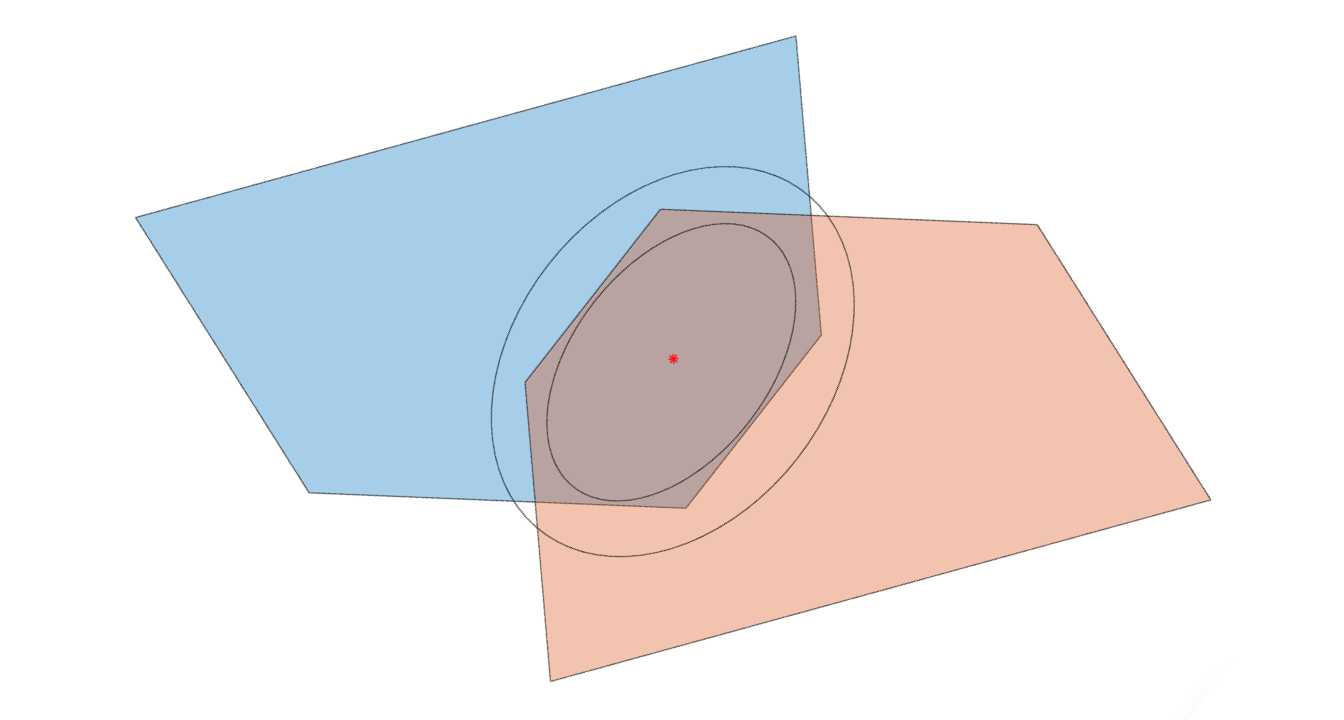
\includegraphics[scale=0.45]{Figures/symmetry}
\par\end{center}%
\end{minipage}\hfill{}%
\begin{minipage}[t]{0.45\textwidth}%
\noindent\begin{flushleft}
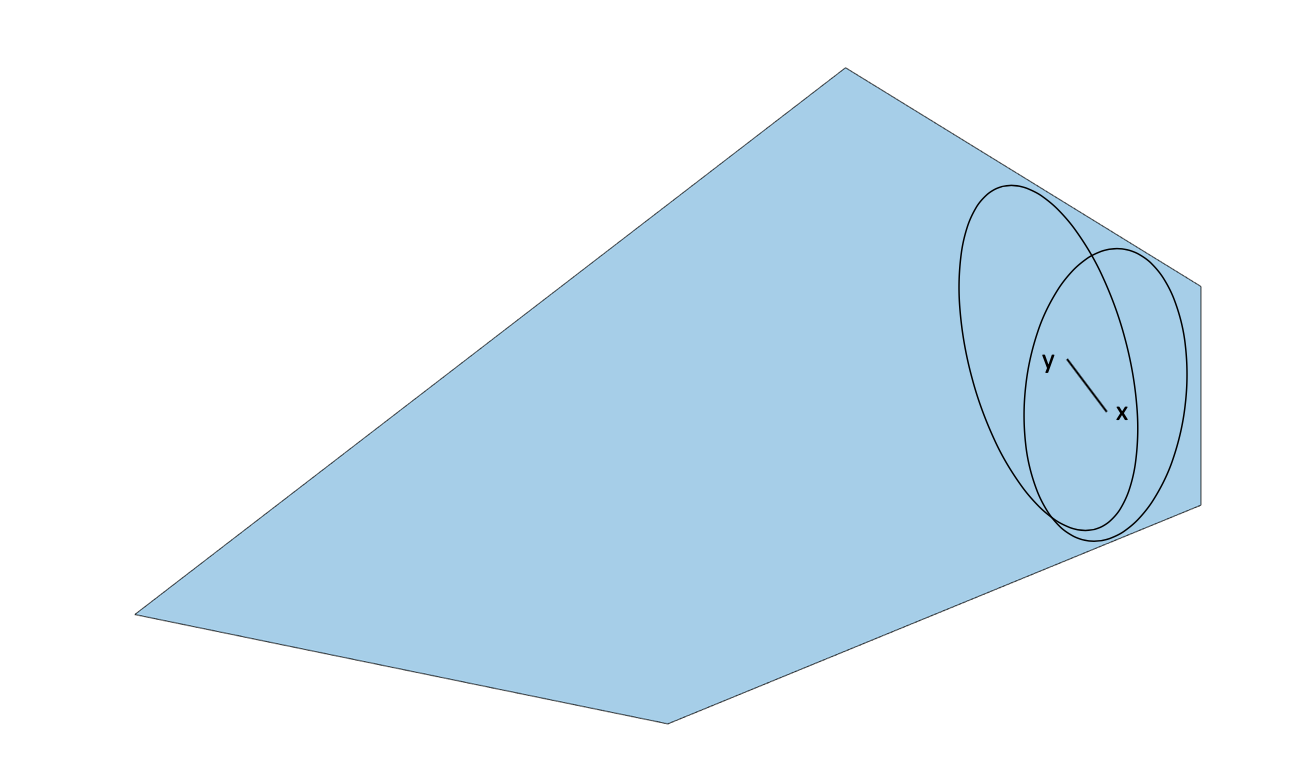
\includegraphics[scale=0.35]{Figures/ssc}
\par\end{flushleft}%
\end{minipage}

\caption{(a) $E_{u}\subseteq K\cap(2u-K)\subseteq\alpha E_{u}.$ (b) Strong
self-concordance measures the rate of change of the Hessian of a barrier
in the Frobenius norm}
\end{figure}
\end{defn}

Similar to Lemma \ref{lem:global_self_concordant}, we have a longer-range
version of stability of the Hessian.
\begin{lem}
\label{lem:global_strongly_self_concordant}Given any strongly self-concordant
matrix function $\mh$ on $K\subset\Rn$, for any $x,y\in K$ with
$\Vert x-y\Vert_{x}<1$, we have
\[
\|\mh(x)^{-\frac{1}{2}}(\mh(y)-\mh(x))\mh(x)^{-\frac{1}{2}}\|_{F}\leq\frac{\|x-y\|_{x}}{(1-\|x-y\|_{x})^{2}}.
\]
\end{lem}

\begin{proof}
Let $x_{t}=(1-t)x+ty$. Then, we have
\begin{align*}
\|\mh(x)^{-\frac{1}{2}}(\mh(y)-\mh(x))\mh(x)^{-\frac{1}{2}}\|_{F} & =\int^{1}_{0}\|\mh(x)^{-\frac{1}{2}}\frac{d}{dt}\mh(x_{t})\mh(x)^{-\frac{1}{2}}\|_{F}dt.
\end{align*}

We note that $\mh$ is self-concordant. Hence, Lemma \ref{lem:global_self_concordant}
shows that
\begin{align*}
\|\mh(x)^{-\frac{1}{2}}\frac{d}{dt}\mh(x_{t})\mh(x)^{-\frac{1}{2}}\|^{2}_{F} & =\tr\mh(x)^{-1}\left(\frac{d}{dt}\mh(x_{t})\right)\mh(x)^{-1}\left(\frac{d}{dt}\mh(x_{t})\right)\\
 & \leq\frac{1}{\left(1-\Vert x-x_{t}\Vert_{x}\right)^{4}}\tr\mh(x_{t})^{-1}\left(\frac{d}{dt}\mh(x_{t})\right)\mh(x_{t})^{-1}\left(\frac{d}{dt}\mh(x_{t})\right)\\
 & \leq\frac{4}{\left(1-\Vert x-x_{t}\Vert_{x}\right)^{4}}\|x-x_{t}\|^{2}_{x_{t}}\\
 & \leq\frac{4}{\left(1-\Vert x-x_{t}\Vert_{x}\right)^{6}}\|x-x_{t}\|^{2}_{x}
\end{align*}

where we used the assumption in the second inequality and Lemma \ref{lem:global_self_concordant}
again for the last inequality. Hence, 
\begin{align*}
\|\mh(x)^{-\frac{1}{2}}(\mh(y)-\mh(x))\mh(x)^{-\frac{1}{2}}\|_{F} & \leq\int^{1}_{0}\frac{2\|x-x_{t}\|_{x}}{\left(1-\Vert x-x_{t}\Vert_{x}\right)^{3}}dt\\
 & =\int^{1}_{0}\frac{2t\|x-y\|_{x}}{(1-t\|x-y\|_{x})^{3}}dt\\
 & =\frac{\|x-y\|_{x}}{(1-\|x-y\|_{x})^{2}}.
\end{align*}
\end{proof}
We note that strong self-concordance can be stronger than self-concordance
since the Frobenius norm is always greater than or equal to the spectral
norm. 
\begin{xca}
Verify that the Hessian of the standard log barrier is strongly self-concordant.
\end{xca}

The main theorem of this section is the following guarantee for the
Dikin walk.
\begin{thm}
\label{thm:dikin}The mixing rate of the Dikin walk with the logarithmic
barrier for a polytope $\{\mathbf{A}x\ge b\}$ is $O(mn)$.
\end{thm}

Each step of the standard Dikin walk can be implemented without using
matrix multiplication.
\begin{thm}
\label{thm:dikin-fast}The Dikin walk with the logarithmic barrier
for a polytope $\{\mathbf{A}x\ge b\}$ can be implemented in time
$O(\nnz(\mathbf{A})+n^{2})$ per step while maintaining the mixing
rate of $O(mn)$.
\end{thm}

A key ingredient of the proof of Theorem \ref{thm:dikin} is the following
lemma.
\begin{lem}
\label{lem:dikin-one-step-1}For two points $x,y\in P$, with $\Vert x-y\Vert_{x}\le\frac{r}{10\sqrt{n}}$,
for $r<0.01$, we have $d_{TV}(P_{x},P_{y})\leq\frac{3}{4}$.
\end{lem}

The proof of this lemma needs several properties captured in the next
exercise.
\begin{xca}
Prove the following for the log barrier in the polytope $\{\mathbf{A}x\ge b\}$:
\end{xca}

\begin{itemize}
\item $\ln\det\mh(x)$ is a convex function.
\item $\Pr_{w\sim E_{x}(r)}\left(\norm{w-x}_{x}\le r\left(1-\frac{1}{n}\right)\right)\ge1-c_{0}r$
for some constant $c_{0}$.
\item $\Pr_{w\sim E_{x}(r)}\left(\norm{w-x}_{w}+\norm{w-x}_{2x-w}\le2r\left(1-\frac{1}{n}\right)\vert\norm{w-x}_{x}\le r\left(1-\frac{1}{n}\right)\right)\ge1-c_{1}r$
for some constant $c_{1}$.
\item $\Pr_{w\sim E_{x}(r)}\left(x\in E_{w}(r)\right)\ge0.5-c_{2}r$ for
some constant $c_{2}$.
\end{itemize}
\begin{proof}[Proof of Lemma \ref{lem:dikin-one-step-1}.]
We have to prove two things: first, the rejection probability is
small, second the ellipsoids used by the Dikin walk at $x,y$ have
large overlap. More precisely, we have
\begin{align}
d_{\mathrm{TV}}(P_{x},P_{y}) & \leq\frac{1}{2}\text{rej}_{x}+\frac{1}{2}\text{rej}_{y}+\frac{1}{2}\frac{\vol(P_{x}\backslash P_{y})}{\vol(P_{x})}+\frac{1}{2}\frac{\vol(P_{y}\backslash P_{x})}{\vol(P_{y})}\nonumber \\
 & =\frac{1}{2}\text{rej}_{x}+\frac{1}{2}\text{rej}_{y}+1-\frac{1}{2}\frac{\vol(P_{x}\cap P_{y})}{\vol(P_{x})}-\frac{1}{2}\frac{\vol(P_{x}\cap P_{y})}{\vol(P_{y})}\label{eq:dikin_formula}
\end{align}
where $\text{rej}_{x}$ and $\text{rej}_{y}$ are the rejection probabilities
at $x$ and $y$.

For the rejection probability at $x$, we consider the algorithm that
picks $z$ from $E_{x}(r)$. Let $f(z)=\ln\det\mathbf{H}(z)$. The
acceptance probability of the sample $z$ is
\begin{equation}
\min\left\{ 1,\frac{\vol(E_{x}(r))}{\vol(E_{z}(r))}\right\} =\min\left\{ 1,\sqrt{\frac{\det(\mathbf{H}(z))}{\det(\mathbf{H}(x))}}\right\} .\label{eq:reject_prob_z}
\end{equation}
By the assumption that $f$ is a convex function, we have that
\begin{equation}
\ln\frac{\det(\mathbf{H}(z))}{\det(\mathbf{H}(x))}=f(z)-f(x)\geq\langle\nabla f(x),z-x\rangle.\label{eq:log_det_Hzx}
\end{equation}
To simplify the notation, we assume $\mh(x)=\mi$. Since $z$ is sampled
from unit ball of radius $r$ centered at $x$, we know that 
\[
\P(v^{\top}(z-x)\geq-\epsilon r\|v\|_{2})\geq1-e^{-n\epsilon^{2}/2}.
\]
In particular, with probability at least $0.99$ in $z$, we have
\begin{equation}
\langle\nabla f(x),z-x\rangle\geq-\frac{4r}{\sqrt{n}}\|\nabla f(x)\|_{2}.\label{eq:grad_prob}
\end{equation}
To compute $\|\nabla f(x)\|^{2}_{2}$, it is easier to compute the
directional derivative of $\nabla f$. Note that 
\begin{align}
\|\nabla f(x)\|_{2} & =\max_{\|v\|_{2}=1}\nabla f(x)^{\top}v\nonumber \\
 & =\max_{\|v\|_{2}=1}\tr(\mh(x)^{-1}D\mh(x)[v])\nonumber \\
 & =\max_{\|v\|_{2}=1}\tr\left(\mh(x)^{-\frac{1}{2}}D\mh(x)[v]\mh(x)^{-\frac{1}{2}}\right)\nonumber \\
 & \leq\max_{\|v\|_{2}=1}\sqrt{n}\|\mh(x)^{-\frac{1}{2}}D\mh(x)[v]\mh(x)^{-\frac{1}{2}}\|_{F}\nonumber \\
 & \leq\sqrt{n}\label{eq:grad_log_H}
\end{align}
where the first inequality follows from $\left|\sum^{n}_{i=1}\lambda_{i}\right|\leq\sqrt{n}\sqrt{\sum^{n}_{i=1}\lambda^{2}_{i}}$
and the second inequality follows from the definition of strong self-concordance.

Combining (\ref{eq:reject_prob_z}), (\ref{eq:log_det_Hzx}), (\ref{eq:grad_prob})
and (\ref{eq:grad_log_H}), we see that with probability at least
$0.99$ in $z$, acceptance probability of the sample $z$, assuming
that $x\in E_{z}(r)$ is 
\begin{equation}
\min\left\{ 1,\frac{\vol(E_{x}(r))}{\vol(E_{z}(r))}\right\} \geq e^{-2r}\geq0.9\label{eq:rejection}
\end{equation}
where we used that $r\le\frac{1}{20}$. Hence the rejection probability
$\mathrm{rej}_{x}$ (and similarly $\mathrm{rej}_{y}$) including
the event $x\in E_{z}(r)$ which happens with probability at least
$0.4$ from the previous exercise, satisfies
\begin{equation}
\mathrm{rej}_{x}\leq0.7\qquad\text{and}\qquad\mathrm{rej}_{y}\leq0.7.\label{eq:rej_xy}
\end{equation}

Now, we bound the fraction of volume in the intersection of the ellipsoids
at $x,y$. Again, we can assume that $\mh(x)=\mi$. Then, strong self-concordance
and Lemma \ref{lem:global_strongly_self_concordant} shows that
\begin{equation}
\|\mh(y)-\mi\|_{F}\leq2\|x-y\|_{x}\leq\frac{1}{10\sqrt{n}}.\label{eq:H_minus_I_F}
\end{equation}
In particular, we have that 
\begin{equation}
0.9\mi\preceq\mh(y)\preceq1.1\mi.\label{eq:H_I_op}
\end{equation}

We partition the eigenvalues $\lambda_{i}$ of $\mh(y)$ into those
of value at least $1$ and the rest. Then consider the ellipsoid $E$
whose eigenvalues are $\min\left\{ 1,\lambda_{i}\right\} $. This
is contained in both $E_{x}(1)$ and $E_{y}(1)$. We will see that
$\vol(E)$ is a constant fraction of the volume of both $E_{x}(1)$
and $E_{y}(1)$. First, we compare $E$ and $E_{x}(1)$
\begin{equation}
\frac{\vol(E)}{\vol(E_{x}(1))}=\prod_{i:\lambda_{i}<1}\lambda_{i}=\prod_{i:\lambda_{i}<1}\left(1-(1-\lambda_{i})\right)\geq\exp\left(-2\sum_{i:\lambda_{i}<1}\left(1-\lambda_{i}\right)\right)\label{eq:vol_E_x}
\end{equation}
where we used that $1-x\geq\exp(-2x)$ for $0\leq x\leq\frac{1}{2}$
and $\lambda_{i}\geq\frac{1}{2}$ (\ref{eq:H_I_op}). From the inequality
(\ref{eq:H_minus_I_F}), it follows that
\[
\sqrt{\sum_{i}(\lambda_{i}-1)^{2}}\le\frac{1}{10\sqrt{n}}.
\]
Therefore, $\sum_{i:\lambda_{i}<1}|\lambda_{i}-1|\leq0.1$. Putting
it into (\ref{eq:vol_E_x}), we have
\begin{equation}
\frac{\vol(P_{x}\cap P_{y})}{\vol(P_{x})}=\frac{\vol(E)}{\vol(E_{x}(1))}\geq e^{-0.2}.\label{eq:volPxyPx}
\end{equation}
Similarly, we have
\begin{equation}
\frac{\vol(P_{x}\cap P_{y})}{\vol(P_{y})}=\frac{\prod_{i:\lambda_{i}<1}\lambda_{i}}{\prod_{i:\lambda_{i}}\lambda_{i}}=\frac{1}{\prod_{i:\lambda_{i}>1}\lambda_{i}}\geq\frac{1}{\exp(\sum_{i:\lambda_{i}>1}(\lambda_{i}-1))}\geq e^{-0.1}.\label{eq:volPxyPy}
\end{equation}

Putting (\ref{eq:rej_xy}), (\ref{eq:volPxyPx}) and (\ref{eq:volPxyPy})
into (\ref{eq:dikin_formula}), we have
\[
d_{\mathrm{TV}}(P_{x},P_{y})\leq\frac{0.7}{2}+\frac{0.7}{2}+1-\frac{e^{-0.2}}{2}-\frac{e^{-0.1}}{2}\leq\frac{3}{4}.
\]
\end{proof}
The other key ingredient for proving the mixing rate is an isoperimetric
inequality. We will in fact use the one for the cross-ratio distance
(Theorem \ref{thm:iso-cross-ratio}) that came up in the analysis
of Hit-and-Run. We can relate the cross-ratio distance to the local
norm induced by the Dikin ellipsoid.
\begin{lem}
\label{lem:dikin-dist-1}For $u,v\in K$, $d_{K}(u,v)\ge\frac{\Vert u-v\Vert_{u}}{\sqrt{m}}$
where $\norm{\cdot}_{u}$ is the norm induced by the Hessian of the
log barrier. 
\end{lem}

The proof will need the following elementary fact about the log barrier.
\begin{lem}
\label{lem:dikin_sandwich}For the Dikin ellipsoid induced by any
self-concordant barrier, we have $E_{x}(1)\subseteq K\cap(2x-K)$
and for the logarithmic barrier for a polytope $K=\{\mathbf{A}x\ge b\}$
defined by $m$ inequalities we also have $K\cap(2x-K)\subseteq E_{x}(\sqrt{m})$.
\end{lem}

\begin{proof}
For the first inequality, we notice that since for any $x\in K$,
we have that the barrier function $\phi$ is finite with bounded first
and second derivatives, and by Lemma \ref{lem:global_self_concordant},
the Hessian remains finite for every point in $[x,y]$ for $y$ such
that $\norm{x-y}_{x}<1$, we have that $\phi(y)$ is also finite,
and hence $y\in K$, since $\phi$ is a barrier function for $K$. 

For the second part, for any $y\in K\cap(2x-K)$, we have that for
every $i\in[m]$, 
\[
\left|a^{\top}_{i}y-a^{\top}_{i}x\right|\le a^{\top}_{i}x-b_{i}
\]
and hence 
\[
\frac{\left|a^{\top}_{i}y-a^{\top}_{i}x\right|}{a^{\top}_{i}x-b_{i}}\le1.
\]
Therefore, 
\[
(y-x)^{\top}\nabla^{2}\phi(x)(y-x)=\sum^{m}_{i=1}\frac{\left(a^{\top}_{i}(y-x)\right)^{2}}{\left(a^{\top}_{i}x-b_{i}\right)^{2}}\le m.
\]
\end{proof}
We can now prove Lemma \ref{lem:dikin-dist-1}.
\begin{proof}[Proof of Lemma \ref{lem:dikin-dist-1}.]
 Consider the ellipsoid at $u$. For the chord $[p,q]$ induced by
$u,v$ with these points in the order $p,u,v,q$, suppose that $\|p-u\|_{2}\le\|v-q\|_{2}$.
Then by Lemma \ref{lem:dikin_sandwich}, $p\in K\cap(2u-K)$. And
hence $\|p-u\|_{u}\le\sqrt{m}.$ Therefore, 
\[
d_{K}(u,v)=\frac{\|u-v\|_{2}\|p-q\|_{2}}{\|p-u\|_{2}\|v-q\|_{2}}\geq\frac{\|u-v\|_{2}}{\|p-u\|_{2}}=\frac{\|u-v\|_{u}}{\|p-u\|_{u}}\ge\frac{\|u-v\|_{u}}{\sqrt{m}}.
\]
\end{proof}
We can now prove the main conductance bound.
\begin{thm}
The conductance of the Dikin walk with the log barrier applied to
a polytope $\{\mathbf{A}x\ge b\}$ with any $r<0.01$ is $\Omega(r/\sqrt{mn})$.
\end{thm}

\begin{proof}
We follow the standard high-level outline. Consider any measurable
subset $S_{1}\subseteq K$ and let $S_{2}=K\setminus S_{1}$ be its
complement. Define the points with low escape probability for these
subsets as:
\[
S_{i}'=\left\{ x\in S_{i}:\,P_{x}(K\setminus S_{i})<\frac{1}{8}\right\} 
\]
and let $S_{3}'=K\setminus S_{1}'\setminus S_{2}'$. Then, for any
$u\in S_{1}'$, $v\in S_{2}'$, we have $d_{TV}(P_{u},P_{v})>1-\frac{1}{4}$.
Hence, by Lemma \ref{lem:dikin-one-step-1}, we have $\Vert u-v\Vert_{u}\ge\frac{r}{10\sqrt{n}}$.
Therefore, by Lemma \ref{lem:dikin-dist-1}, 
\[
d_{K}(u,v)\ge\frac{r}{10\sqrt{n}\cdot\sqrt{m}}.
\]
We can now bound the conductance of $S_{1}$. We may assume that $\vol(S_{i}')\ge\vol(S_{i})/2$;
otherwise, it immediately follows that the conductance of $S_{1}$
is $\Omega(1)$. Assuming this, we have
\begin{align*}
\int_{S_{1}}P_{x}(S_{2})\,dx & \ge\frac{1}{2}\int_{S_{3}'}\frac{1}{8}dx\ge\frac{1}{16}\vol(S_{3}')\\
 & \ge\frac{1}{16}d_{K}(S_{1}',S_{2}')\frac{\vol(S_{1}')\vol(S_{2}')}{\vol(P)}\qquad\text{(Theorem \ref{thm:iso-cross-ratio})}\\
 & \ge\frac{r}{1000\sqrt{nm}}\min\left\{ \vol(S_{1}),\vol(S_{2})\right\} .
\end{align*}
\end{proof}

